\chapter{Introduction}
\section{Notation}

\section{Block ciphers}

Securing communication channels between different parties has been a long-term
subject of study for cryptographers and engineers which is essential to our
modern world to cope with ever-increasing amounts of devices producing and
sharing data. The main way to facilitate high-throughput, confidential
communications nowadays is through the use of symmetric cryptography in which
two parties share a common secret, called a key, which allows them to encrypt,
share and subsequently decrypt messages to achieve confidentiality against
third parties. Ciphers can be divided into two categories; block ciphers, which
always encrypt fixed-sized messages called blocks, and stream ciphers, which
continuously provide encryption for an arbitrarily long, constant stream of
data.

A block cipher can be defined as a bijection between the input block (the
message) and the output block (the ciphertext). For any block cipher with block
size $n$, we denote the key-dependent encryption and decryption functions as
$E_K,D_K:\F{n}\rightarrow \F{n}$. The simplest way to
characterize this bijection is through a lookup table which yields the highest
possible performance as each block can be encrypted by one simple lookup
depending on the key and the message. This is not practical though due to most
ciphers working with block and key sizes $n,|K|\geq 64$. For a block cipher
with $n=64,|K|=128$, a space of $2^{64}2^{128}64=2^{198}$ is necessary.
Considering modern consumer hard disks being able to store data in the order of
$2^{40}$, it is easy to see that a lookup table is wholly impractical. We
therefore describe block ciphers algorithmically which opens up possibilities
for different tradeoffs and security concerns.


\subsection{GIFT}

\texttt{GIFT}\cite{gift:2017}, first presented in the \textit{CHES 2017}
cryptographic hardware and embedded systems conference, is a lightweight block
cipher based on a previous design called \texttt{PRESENT}, developed in 2007. Its
goal is to offer maximum security while being extremely light on resources.
Modern battery-powered devices like RFID tags or low-latency operations like
on-the-fly disc encryption present strong hardware and power constraints. GIFT
aims to be a simple, low-energy cipher suited for these kinds of applications.

\texttt{GIFT} comes in two variants; \verb|GIFT-64| working with 64-bit blocks
and \texttt{GIFT-128} working with 128-bit blocks. In both cases, the key is 128
bits long. The design is a very simple, round-based substitution-permutation
network (SPN). One round consists in a sequential application of the confusion
layer by means of 4-bit S-boxes and subsequent diffusion through bit
permutation. After the bit permutation, a round key is added to the cipher
state and the single round is complete. \texttt{GIFT-64} uses 28 rounds while
\texttt{GIFT-128} uses 40 rounds.

\begin{figure}[h!]
    \centering
    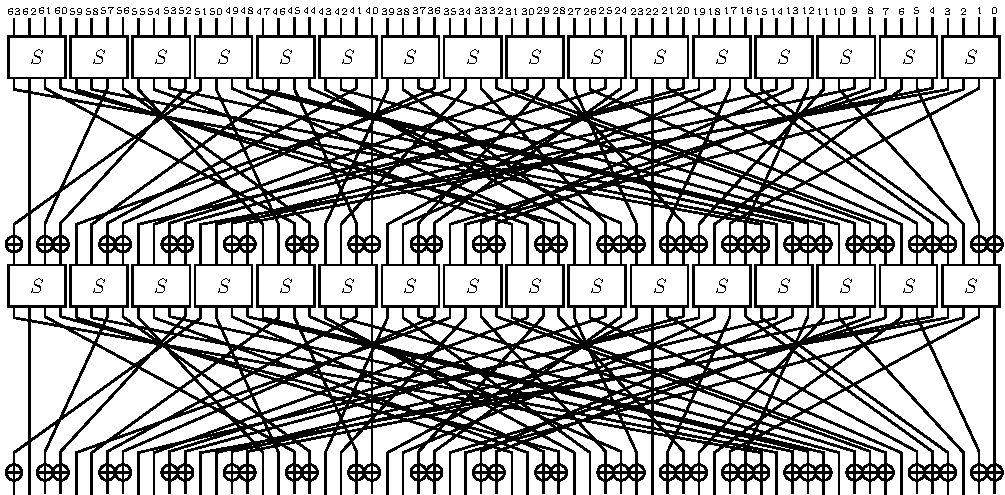
\includegraphics[width=\textwidth]{Figures/GIFT-64.pdf}
    \caption{Two rounds of GIFT-64}
\end{figure}

\subsubsection{Substitution layer}

The input of \texttt{GIFT} is split into 4-bit nibbles which are then fed into
16 S-boxes for \texttt{GIFT-64} and 32 S-boxes for \texttt{GIFT-128}. The S-box
$S:\F{4}\rightarrow \F{4}$ is defined as follows:

\[
    \begin{array}{l|cccccccccccccccc}
        x & 0 & 1 & 2 & 3 & 4 & 5 & 6 & 7 & 8 & 9 & a & b & c & d & e & f \\
        \hline
        S(x) & 1 & a & 4 & c & 6 & f & 3 & 9 & 2 & d & b & 7 & 5 & 0 & 8 & e
    \end{array}
\]

\subsubsection{Permutation layer}

The permutation $P$ works on individual bits and maps bit $b_i$ to $b_{P(i)},
i\in\{0,1,\dots,n-1\}$. The different permutations for \texttt{GIFT-64} and
\texttt{GIFT-128} can be expressed by:

\begin{align*}
    P_{64}(i)&=4\left\lfloor\frac{i}{16}\right\rfloor+16\left(\left(3\left\lfloor\frac{i\bmod 16}{4}\right\rfloor+(i\bmod 4)\right)\bmod 4\right)+(i\bmod 4) \\
    P_{128}(i)&=4\left\lfloor\frac{i}{16}\right\rfloor+32\left(\left(3\left\lfloor\frac{i\bmod 16}{4}\right\rfloor+(i\bmod 4)\right)\bmod 4\right)+(i\bmod 4) \\
\end{align*}

\subsubsection{Round key addition}

The last step of each round consists in XORing a round key $R_i$ to the cipher
state. The new cipher state $s_{i+1}$ after each full round is therefore given
by

\[
    s_{i+1}=P(S(s_i))\oplus R_i
\]

\subsubsection{Round key extraction and key schedule}

Round key extraction differs for \texttt{GIFT-64} and \texttt{GIFT-128}. Let
$K=k7||k6||\dots||k0$ denote the $128$-bit key state.

\paragraph{GIFT-64}. We extract two 16-bit words $U||V=k_1||k_0$ from the key
state. $u_i$ and $v_i$ are XORed to $r_{4i+1}$ and $r_{4i}$ of the round key
$R$ respectively.

\paragraph{GIFT-128}. We extract two 32-bit words $U||V=k_5||k4||k1||k_0$ from
the key state. $u_i$ and $v_i$ are XORed to $r_{4i+2}$ and $b_{4i+1}$ of the
round key $R$ respectively.

In both cases, we additionally XOR a round constant $C=c_5c_4c_3c_2c_1c_0$ to
bit positions $n-1,23,19,15,11,7,3$. The round constants are generated using a
6-bit affine linear-feedback shift register and have the following values:\\

\begin{tabular}{r|l}
    \textbf{Rounds} & \textbf{Constants} \\
    \hline
    \textbf{1 - 16} &  \small\texttt{01,03,07,0F,1F,3E,3D,3B,37,2F,1E,3C,39,33,27,0E} \\
    \textbf{17 - 32} & \small\texttt{1D,3A,35,2B,16,2C,18,30,21,02,05,0B,17,2E,1C,38} \\
    \textbf{33 - 48} & \small\texttt{31,23,06,0D,1B,36,2D,1A,34,29,12,24,08,11,22,04}
\end{tabular}\\

The key state is then updated by setting $k_1\leftarrow k_1\ggg 2$,
$k_0\leftarrow k_0\ggg 12$ and rotating the new state $32$ bits to the right:

\[
    k_7||k_6||\dots||k_1||k_0\leftarrow k_1\ggg 2||k_0\ggg 12||k_7||k_6||\dots||k_3||k_2
\]

\subsection{Camellia}

\section{The ARMv8 platform}

With small devices, embedded processors and ASICs becoming ever more ubiquitous
and essential in areas like medicine or automotive design, the need for ...
